\documentclass[border=3pt]{standalone}
% Preâmbulo compartilhado pelos diagramas TikZ da aula 4 de Navegação (Representação de Mapas)
\usepackage[T1]{fontenc}
\usepackage[utf8]{inputenc}
\usepackage{lmodern}
\usepackage{amsmath}
\usepackage{xcolor}
\usepackage{tikz}
\usetikzlibrary{arrows.meta,angles,quotes,decorations.pathmorphing,decorations.pathreplacing,calc,
                positioning,shapes.geometric,shapes.misc,backgrounds,fit,
                math}

% Paleta (mesma dos SVGs originais)
\definecolor{dblue}{HTML}{2A5B8C}
\definecolor{dorange}{HTML}{B3541E}
\definecolor{dgreen}{HTML}{4A7C59}
\definecolor{dred}{HTML}{9C4B4B}
\definecolor{dcream}{HTML}{F4F1EA}
\definecolor{dshade}{HTML}{DDD7C9}

% Função gaussiana (não normalizada por padrão de escala visual)
\pgfmathdeclarefunction{gauss}{3}{%
  \pgfmathparse{1/(#3*sqrt(2*pi))*exp(-((#1-#2)^2)/(2*#3^2))}%
}

% Estilos comuns (prefixo d... para não colidir com chaves internas do pgf)
\tikzset{
  >={Stealth[length=2mm]},
  dguide/.style={gray!55, dashed, line width=0.4pt},
  daxis/.style={gray!60, line width=0.7pt, ->},
  dbody/.style={fill=black!3, draw=black!80, line width=1pt},
  dacc/.style={draw=dblue, line width=1pt},
  dlbl/.style={black!55, font=\small},
  dsub/.style={black!45, font=\footnotesize},
  dstate/.style={circle, draw=black!80, fill=dcream, line width=1pt,
                 minimum size=17mm, font=\large, inner sep=1pt},
  dobs/.style={circle, draw=black!80, fill=dshade, line width=1pt,
               minimum size=14mm, font=\large, inner sep=1pt},
  dbox/.style={rounded corners=2pt, draw=black!80, fill=dcream, line width=1pt,
               align=center, inner sep=6pt},
  dop/.style={circle, draw=black!80, fill=white, line width=1pt,
              minimum size=6mm, inner sep=0pt, font=\small},
  dtrans/.style={->, dblue, line width=1pt},
  dmeas/.style={->, dorange, line width=1pt},
  dcurve/.style={line width=1pt, dblue},
  dcurveb/.style={line width=1.4pt, dorange},
}

\begin{document}
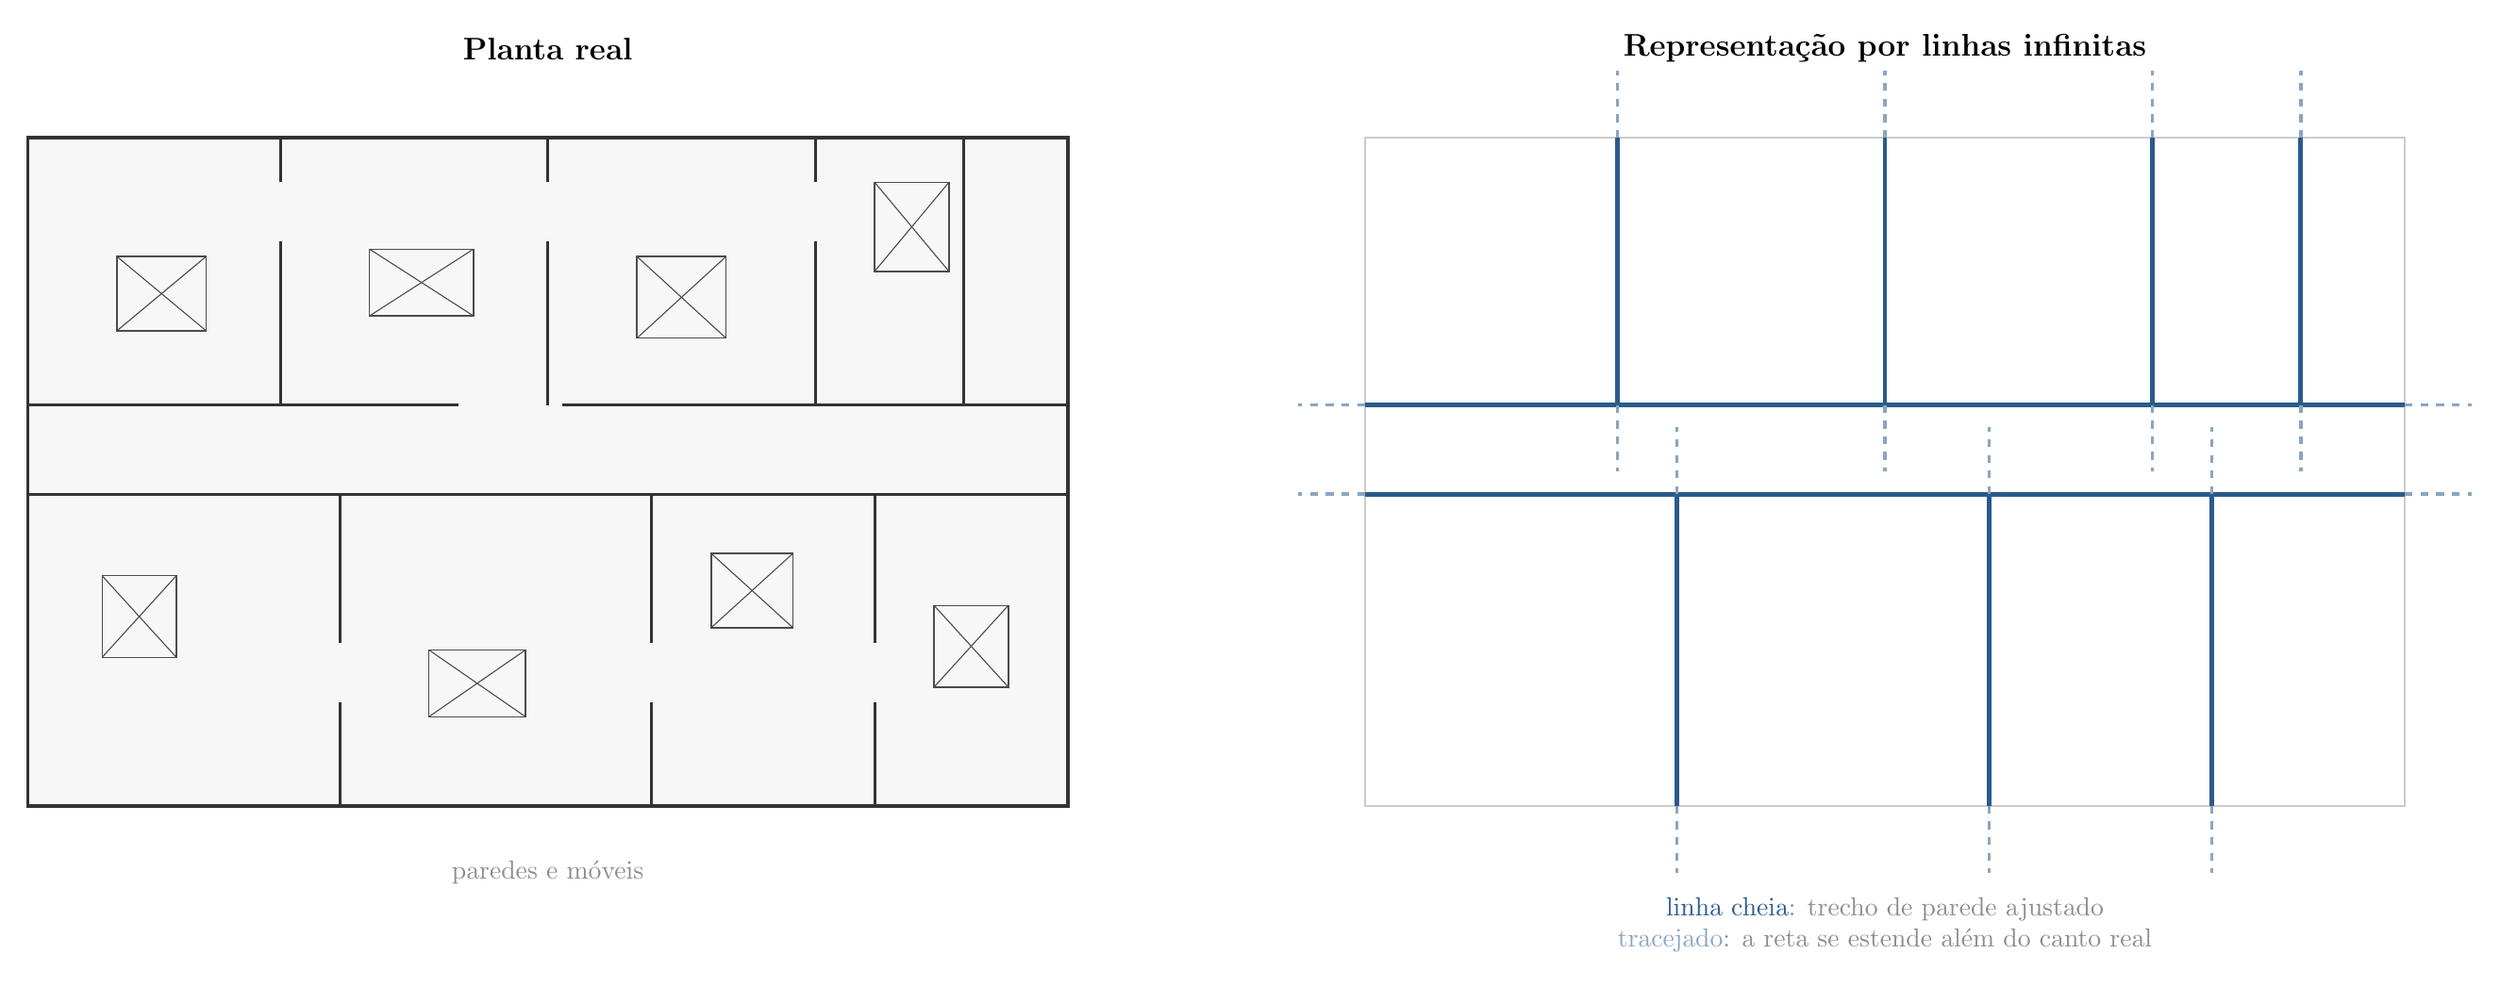
\begin{tikzpicture}[x=1cm,y=1cm]

  \begin{scope}
    \node[font=\bfseries\large] at (7,10.2) {Planta real};
    \draw[dbody, line width=1.3pt] (0,0) rectangle (14,9);
    \draw[dbody, line width=1.1pt] (0,4.2) -- (14,4.2);
    \draw[dbody, line width=1.1pt] (0,5.4) -- (5.8,5.4);
    \draw[dbody, line width=1.1pt] (7.2,5.4) -- (14,5.4);
    \draw[dbody, line width=1.1pt] (3.4,5.4) -- (3.4,7.6) (3.4,8.4) -- (3.4,9);
    \draw[dbody, line width=1.1pt] (7.0,5.4) -- (7.0,7.6) (7.0,8.4) -- (7.0,9);
    \draw[dbody, line width=1.1pt] (10.6,5.4) -- (10.6,7.6) (10.6,8.4) -- (10.6,9);
    \draw[dbody, line width=1.1pt] (12.6,5.4) -- (12.6,9);
    \draw[dbody, line width=1.1pt] (4.2,0) -- (4.2,1.4) (4.2,2.2) -- (4.2,4.2);
    \draw[dbody, line width=1.1pt] (8.4,0) -- (8.4,1.4) (8.4,2.2) -- (8.4,4.2);
    \draw[dbody, line width=1.1pt] (11.4,0) -- (11.4,1.4) (11.4,2.2) -- (11.4,4.2);
    \foreach \x/\y/\w/\h in {1.2/6.4/1.2/1.0, 4.6/6.6/1.4/0.9, 8.2/6.3/1.2/1.1, 11.4/7.2/1.0/1.2, 1.0/2.0/1.0/1.1, 5.4/1.2/1.3/0.9, 9.2/2.4/1.1/1.0, 12.2/1.6/1.0/1.1} {
      \draw[black!70, line width=0.5pt] (\x,\y) rectangle ++(\w,\h);
      \draw[black!70, line width=0.4pt] (\x,\y) -- ++(\w,\h);
      \draw[black!70, line width=0.4pt] (\x+\w,\y) -- ++(-\w,\h);
    }
    \node[dsub, font=\normalsize] at (7,-0.9) {paredes e móveis};
  \end{scope}
\begin{scope}[shift={(18,0)}]
\node[font=\bfseries\large] at (7,10.2) {Representação por linhas infinitas};
\draw[black!20, line width=0.6pt] (0,0) rectangle (14,9);
\draw[dblue, line width=1.8pt] (0.00,4.20) -- (14.00,4.20);
\draw[dblue!55, dash pattern=on 3pt off 3pt, line width=1.2pt] (0.00,4.20) -- (-0.90,4.20);
\draw[dblue!55, dash pattern=on 3pt off 3pt, line width=1.2pt] (14.00,4.20) -- (14.90,4.20);
\draw[dblue, line width=1.8pt] (0.00,5.40) -- (14.00,5.40);
\draw[dblue!55, dash pattern=on 3pt off 3pt, line width=1.2pt] (0.00,5.40) -- (-0.90,5.40);
\draw[dblue!55, dash pattern=on 3pt off 3pt, line width=1.2pt] (14.00,5.40) -- (14.90,5.40);
\draw[dblue, line width=1.8pt] (3.40,5.40) -- (3.40,9.00);
\draw[dblue!55, dash pattern=on 3pt off 3pt, line width=1.2pt] (3.40,5.40) -- (3.40,4.50);
\draw[dblue!55, dash pattern=on 3pt off 3pt, line width=1.2pt] (3.40,9.00) -- (3.40,9.90);
\draw[dblue, line width=1.8pt] (7.00,5.40) -- (7.00,9.00);
\draw[dblue!55, dash pattern=on 3pt off 3pt, line width=1.2pt] (7.00,5.40) -- (7.00,4.50);
\draw[dblue!55, dash pattern=on 3pt off 3pt, line width=1.2pt] (7.00,9.00) -- (7.00,9.90);
\draw[dblue, line width=1.8pt] (10.60,5.40) -- (10.60,9.00);
\draw[dblue!55, dash pattern=on 3pt off 3pt, line width=1.2pt] (10.60,5.40) -- (10.60,4.50);
\draw[dblue!55, dash pattern=on 3pt off 3pt, line width=1.2pt] (10.60,9.00) -- (10.60,9.90);
\draw[dblue, line width=1.8pt] (12.60,5.40) -- (12.60,9.00);
\draw[dblue!55, dash pattern=on 3pt off 3pt, line width=1.2pt] (12.60,5.40) -- (12.60,4.50);
\draw[dblue!55, dash pattern=on 3pt off 3pt, line width=1.2pt] (12.60,9.00) -- (12.60,9.90);
\draw[dblue, line width=1.8pt] (4.20,0.00) -- (4.20,4.20);
\draw[dblue!55, dash pattern=on 3pt off 3pt, line width=1.2pt] (4.20,0.00) -- (4.20,-0.90);
\draw[dblue!55, dash pattern=on 3pt off 3pt, line width=1.2pt] (4.20,4.20) -- (4.20,5.10);
\draw[dblue, line width=1.8pt] (8.40,0.00) -- (8.40,4.20);
\draw[dblue!55, dash pattern=on 3pt off 3pt, line width=1.2pt] (8.40,0.00) -- (8.40,-0.90);
\draw[dblue!55, dash pattern=on 3pt off 3pt, line width=1.2pt] (8.40,4.20) -- (8.40,5.10);
\draw[dblue, line width=1.8pt] (11.40,0.00) -- (11.40,4.20);
\draw[dblue!55, dash pattern=on 3pt off 3pt, line width=1.2pt] (11.40,0.00) -- (11.40,-0.90);
\draw[dblue!55, dash pattern=on 3pt off 3pt, line width=1.2pt] (11.40,4.20) -- (11.40,5.10);
\node[dsub, font=\normalsize, align=center] at (7,-1.6) {\textcolor{dblue}{linha cheia}: trecho de parede ajustado\\ \textcolor{dblue!55}{tracejado}: a reta se estende além do canto real};
\end{scope}
\end{tikzpicture}
\end{document}
